\documentclass[12pt, dvipsnames, a4paper]{article}
\usepackage{geometry}
\geometry{legalpaper, margin=0.5in}
\usepackage{xcolor}
\usepackage{lipsum,etoolbox}
\usepackage{xspace} 
\usepackage[normalem]{ulem}
\usepackage{vwcol}
\usepackage{cancel}
\usepackage{enumitem}
\usepackage{amsmath}
\usepackage{caption}
\usepackage{graphicx}
\usepackage{amsfonts}
\usepackage{float}
\usepackage{multicol}
\usepackage{hyperref}
\usepackage{listings}
\usepackage{textcomp}
\usepackage{lstautogobble}
\usepackage[parfill]{parskip}
\usepackage{tikz-qtree}
\usepackage{tikz}
\usepackage{hyperref}
\usepackage[english]{babel}
\usepackage[autostyle, english = american]{csquotes}
\MakeOuterQuote{"}
\usetikzlibrary{decorations.pathreplacing}
\tikzset{every tree node/.style={minimum width=4cm,draw,circle},
         blank/.style={draw=none},
         edge from parent/.style=
         {draw,edge from parent path={(\tikzparentnode) -- (\tikzchildnode)}},
         level distance=1.5cm}

%% Genearl %%
\renewcommand{\thesection}{\arabic{section}}


%% For convenience %%
\newcommand{\code}[1]{\texttt{#1}}
\newcommand{\bcode}[1]{\texttt{\textbf{#1}}}
\newcommand{\balert}[1]{\textbf{\alert{#1}}}
\newcommand{\rarrow}{$\Rightarrow$}
\newcommand{\tab}[1][0.5cm]{\hspace*{#1}}
\newcommand{\deepemphasis}[1]{\underline{\textbf{\Large{#1}}}}
\newcommand{\bfemph}[1]{\textbf{\emph{#1}}}
\newcommand{\OR}[0]{\lvert \: \rvert}

%% Colours %%
\definecolor{mLightBrown}{HTML}{EB811B}
\definecolor{mLightGreen}{HTML}{14B03D}

%% Pseudocode %% 
\lstdefinelanguage{pseudo}
{
	keywords=[1]{
		let,
		class,
		new,
		loop,
		until,
		end,
		if,
		else,
		then,
		return,
		while,
		for,
		to,
		fun,
		break,
		and,
		true,
		false,
		or,
		do,
		max,
		min,
		elif,
	},
	keywordstyle=[1]\color{black}\bf,
	keywords=[2] {
		invariant,
		precond,
		postcond
	},
	keywordstyle=[2]\color{blue}\bf
}

\lstset{
	breaklines		=	true,
	language 		= 	pseudo,
	basicstyle		=	\ttfamily,
	mathescape		=	true,
	escapeinside	=	||,
	tabsize			=	2,
	numbers			=	left,
	commentstyle	=	\color{OliveGreen},
	stringstyle		=	\color{mLightBrown},
	upquote			=	true,
	morestring		=	[b]',
	moredelim		=	[l][\rmfamily\itshape]{@},
	comment			=	[l]{//},
	morecomment		=	[s]{/*}{*/},
	commentstyle=\color{Gray}\ttfamily,
	showstringspaces=	false,
	showtabs		=	false,
	autogobble
}

%% Other %%
\setcounter{secnumdepth}{5}
\setcounter{tocdepth}{5}

% \patchcmd{<cmd>}{<search>}{<replace>}{<success>}{<failure>}
\patchcmd{\abstract}{\titlepage}{\titlepage% Insert ToC-writing after starting a titlepage
  \addcontentsline{toc}{chapter}{Abstract}}{}{}
\setcounter{secnumdepth}{3}
\setcounter{tocdepth}{3}

% Keywords command
\providecommand{\keywords}[1]
{
  \small	
  \textbf{\textit{Keywords---}} #1
}


%**************************************************************************************************************%
%______________________________________________________________________________________________________________%
\begin{document}
\title{\textbf{EECS 4314 - Bit Theory\\Architecture Enhancement Report}}
\date{\Large \today}
\author{
	\large \textbf{Amir Mohamad}\\ \small amohamad@my.yorku.ca\\\\
	\large \textbf{Arian Mohamad Hosaini}\\ \small mohama23@my.yorku.ca\\\\
	\large \textbf{Dante Laviolette}\\ \small dantelav@my.yorku.ca\\\\
	\large \textbf{Diego Santosuosso Salerno}\\ \small nicodemo@my.yorku.ca\\\\
	\large \textbf{Isaiah Linares}\\ \small isaiah88@my.yorku.ca\\\\
	\large \textbf{Joel Fagen}\\ \small joefagan@my.yorku.ca\\\\
	\large \textbf{Misato Shimizu}\\ \small misato1@my.yorku.ca\\\\
	\large \textbf{Muhammad Hassan}\\ \small furquanh@my.yorku.ca\\\\
	\large \textbf{Yi Qin}\\ \small aidenqin@my.yorku.ca\\\\
	\large \textbf{Zhilong Lin}\\ \small lzl1114@my.yorku.ca\\\\
	\large York University\\
}
\maketitle
\newpage
\hspace{0pt}
\vfill
\begin{abstract}
	This report proposes the development of a new feature for the Docker system. This new feature is the implementation of Cgroup and Namespace API for FreeBSD. At the moment, Docker's performance depends on the Linux operating system's Cgroup and Namespace features. By creating a FreeBSD equivalent of these capabilities, Docker may be made to function seamlessly on the platform, expanding its user base and increasing its general adaptability.

	The suggested improvement will be thoroughly covered, including its potential value and advantages for different stakeholders. We'll look at the architectural adjustments needed to accommodate this functionality, paying particular attention to the high-level parts and interfaces that need to change. The study will examine how this new feature interacts with existing functionality and give a thorough comparison of the system's current and improved states.

	Additionally, the study will examine how this architectural change will affect both high-level and low-level system concepts, with the help of an architecture diagram that graphically illustrates the changes. The discussion of flagged files, use cases, and concurrency issues will also be included to ensure that all aspects of the proposed improvement are clear.

	The implementation of the Cgroup and Namespace API for FreeBSD will be assessed for potential risks and constraints, identifying any potential negative outcomes. The study will end with a summary of the results and an evaluation of the feasibility and advantages of adding this improvement to the Docker software system overall.
	\newline
	\keywords{cgroups, namespaces, containerization, Docker, compatibility}
\end{abstract}
\vfill
\hspace{0pt}
\newpage
\tableofcontents
\clearpage

\section{Introduction}
\subsection{Problem Definition}
FreeBSD currently relies on jails for providing containerization capabilities. However, as containerization needs evolve, the limitations of jails become more evident.
Jails work well for simple isolation use cases but lack features critical for more advanced container workflows. They provide a basic level of encapsulation but lack the portability and interoperability of modern container formats. Jails also have limited options for networking, storage, and orchestration between containers.
Additional container tools are needed to address these limitations and meet the growing demands of containerized applications and infrastructure. Options like Kubernetes are attracting developers and sysadmins to containerized platforms but FreeBSD remains limited to jails.

Integration with other open source container projects would make FreeBSD far more suitable for the microservices, cloud-native environments, and CI/CD pipelines that are increasingly prevalent. When combined with FreeBSD's security, stability and customizability, new container technologies could significantly expand usage possibilities.

With containerization becoming integral to application development and deployment, FreeBSD requires further enhancements beyond just jails. Options for container formats, networks, storage, and orchestration would provide far more flexibility and capabilities. Developing or leveraging additional tools would position FreeBSD as a robust, configurable operating system able to support containerized workloads at scale.

Advancements in containerization are essential for FreeBSD to meet evolving needs and remain competitive. Jails alone no longer suffice for the kinds of containerized architectures and workflows common today. Additional container tools will be needed to address limitations, unlock new potential, and ensure FreeBSD keeps pace with rapid changes in containerization. Keeping up with container futures will require more possibilities beyond just jails.

\subsection{Docker}
Docker is a famous software that uses OS-level virtualization to deliver software in packages called containers. It has been widely used in many mainstream operating systems such as Windows, macOS, and Linux. Sadly, Docker can't operate on FreeBSD due to the difference in kernel features. Though the Jails in FreeBSD have similar functions as Docker, most users think that Docker works much better than Jails. In fact, Docker performs better than Jails in almost all categories except startup time. As a result, it's reasonable to try to make Docker work on FreeBSD.
To reach our target of allowing features like Docker to be functional in FreeBSD, there are many different approaches. For example, we can run a Linux Virtual Machine within FreeBSD, so that we can containerize without using Jails. However, this will surely be an unnecessary move. Among all those approaches, the one we choose to use to solve the problem is implementing cgroup and namespace 'like' APIs that internally use jails. In Linux, docker requires cgroup and namespace, which are featured on the Linux kernel, to run. What we want is to implement a clone of cgroup and namespace for FreeBSD, so that we can get a result of running Docker on FreeBSD.

\subsection{Overview}

To clearly introduce our project from multi-angel, the report has been divided into six different chapters:
\begin{itemize}
	\item Enhancement - This part explains how the project works and explains the benefits it brings.
	\item Stakeholders - Show the influence that might happen to developers, users, and other stakeholders.
	\item Architectural Impact - This part shows the concrete architecture changes caused by the enhancements through diagrams.
	\item Concurrency - Compares concurrency of different versions of cgroup in Linux.
	\item Risk \& Limitation - Find out the risk and limitations that might appear.
	\item Conclusion - Summarize the whole report and record the lessons learned in the process.
\end{itemize}
\clearpage


\section{Enhancement}
\subsection{Our Proposed Enhancement}
Our proposed enhancement is to extend the current Linux emulator for FreeBSD, Linuxulator, to also handle cgroup and namespace calls. Currently they are not implemented because they are features that act on hardware and can’t be directly mapped to a FreeBSD system calls. This causes problems with many Linux binaries that utilize cgroups or namespaces as well as Container runtimes which are used widely in Linux development. After this interface is added almost all binaries will now run easily using the Linuxulator, which is important because Linux is heavily supported and has a lot of developers making useful binaries. Another benefit is that OCI compliant container run-times like runc, Containerd, or Docker would work natively instead of using ports. The port for running OCI compliant runtimes, runj, utilizes jails to make Containers and is currently under development. This works great natively for FreeBSD but the goal is to integrate FreeBSD into the broader Docker ecosystem and using our interface would allow widely used OCI runtimes to work seamlessly and remove complication.

\subsection{Alternatives}
For many Linux binaries running through Linuxulator there aren't any great alternatives to this interface, as cgroup and namespaces are very integral to some programs. It is possible to edit Linux binaries through FreeBSD but this can cause the Linux binary to use a lot of efficiency or functionality. A more viable solution is to use a Linux Virtual machine inside FreeBSD, which allows you to run any Linux binary and use all types of OCI runtimes like Docker, Containerized, runc, etc… Although a lot of developers will not like this method as it brings a lot of overhead which will slow down Linux binaries. This is something Linux developers will not tolerate because the main reason people use Linux operating systems is because it removes overhead and allows them to work more efficiently!. This is why our solution is favorable to many developers.

\section{Stakeholders}
With this new implementation of Namespace and Cgroups for FreeBSD several stakeholders who would be involved.

\subsection{Developers}
The first stakeholder is the developers who are working to implement this new improvement as they will be the ones responsible for creating code that will enable docker to run on the FreeBSD platform.Their work will require expertise in kernel architecture, API design, and programming languages like C and Rust, among others.

\subsection{Users}
Secondly, users of Docker who want to use the platform FreeBSD are another stakeholder group. These users, who want to leverage Docker's capabilities on the FreeBSD platform, could be freelance developers, small businesses, or bigger corporations. They might be interested in how Cgroup and Namespace API implementation will affect performance, stability, or security.

\subsection{Docker}
Thirdly the Docker company would also be another key stakeholder. By supporting the FreeBSD platform, they will get the chance to increase their user base. The strategic market expansion or rivalry with competing containerization platforms may be the driving forces behind Docker's involvement in this project.

\subsection{FreeBSD Community}
The FreeBSD community is also a stakeholder group. The Cgroup and Namespace API would improve FreeBSD's functionality and make it a more desirable platform for users and developers. The project might also spark more interest in the FreeBSD operating system, which might result in additional contributions to the open-source initiative or a rise in the use of FreeBSD in commercial settings.

\section{Architecture}
\subsection{Current State of The System}

In the current state of the system, the Linuxulator subsystem provides kernel
interfaces identical to Linux system calls to allow for emulation \cite{linuxbinarycompat}.
It does this by mapping Linux system calls to their FreeBSD equivalents \cite{linuxulator},
while also emulating parts of the Linux filesystem using \texttt{linsysfs} \cite{linsysfs}
Due to this, many Linux binaries can run natively on FreeBSD if the
\texttt{linux\_enable} flag is enabled in \texttt{/etc/rc.conf}.\\

Although, Linuxulator currently doesn't support \texttt{cgroups} or \texttt{namespaces}.
Due to this, any binaries that rely on these Linux features cannot run
natively on FreeBSD without modifications.\\

With that being said, it's important to note that FreeBSD has \texttt{jails},
which cover most of the use-cases of \texttt{cgroups} and \texttt{namespaces}.
A \texttt{jail} provides containerization, while \texttt{namespaces} and \texttt{cgroups}
can be used together to enable containerization.

\subsection{Enhanced State of The System}

Our proposal is to extend Linuxulator to provide interfaces for \texttt{namespaces}
and \texttt{cgroups}, while using \texttt{jails} internally.\\

More specifically, \texttt{namespaces} will be supported by supporting
the \texttt{set\_tid} argument in the \texttt{linux\_clone3} system call (\href{https://github.com/freebsd/freebsd-src/blob/953efa5b200f060564a090ab71b3d7f614a35e3f/sys/compat/linux/linux_fork.c#L398}{\texttt{sys/compat/linux/linux\_fork.c}})
which is currently ignored. Then when the \texttt{CLONE\_NEWPID} flag is passed in
\texttt{set\_tid}, a new jail will be created, which will enable
namespaces \cite{clone}. Internally, some logic will handle mapping the jail ID to the
returned PID, and simulate the cloned process seeing itself as PID 0.\\

The \texttt{cgroups} virtual file system will then be supported in the
Linuxulator file system (\texttt{linsysfs}), which will act as an interface
for modifying the \texttt{jails} resources.\\

With that being said, this will cause the Linuxulator to become dependent on
jails. Although, it will also greatly improve compatibility with linux
binaries, allowing applications such as Docker to run natively, while still
taking advantage of \texttt{jails}.

\subsection{Interactions with Other Features}
In this part, we will be discussing about the impact of interaction and design patterns after
adding these features. We know that Cgroups allows the system administrator to allocate
system resources and place limits on resource usage. First, it will interact with the virtual
memory subsystem to create a more secured system environment. It can be used to limit the
amount of memory being used and preventing it from consuming excessive system resources.
The second interacting part can be security subsystem. Cgroups can be used in conjunction with
other security mechanisms. For example, with the Mandatory Access Control, it can prevent
unauthorized access to system resource. There will be two design patterns can be found in this
feature. It will use command pattern to implement the functionalities and improve the system
performance. Another pattern that scan be found is the builder pattern. It is good for customize
Cgroups for different applications and use cases. It can also make it easier to create and
manage complex configurations.
Namespace is a feature allows for the creations of isolated environments that have their own
independent view of certain system resources including process IDs, network interfaces, file
systems, user IDs, and other system resources. It will be interacted with the process
management system. Namespaces can be used to create isolated process trees so the process
can be limited into smaller parts. Second interacting part can be file system. Namespaces can
be used to isolate files systems between different processes. It can prevent the applications
from accessing or modifying files outside their own namespaces. The design pattern might be
found is proxy pattern. Since it will create an independent view of certain system resource,
using proxy pattern can allow the system to create a virtualized view of the system that is
isolated from the underlying system. It will make it easier and safer to customize the behavior
of the virtualized system.
\clearpage

\subsection{Effect of the Enhancement on the Concrete Architecture}
The Linulator subsystem resides in the newly discovered subsystem called \emph{Compat}, or the Compatibility subsystem. Enhancing FreeBSD for native Docker support by extending the linuxulator subsystem but keeping jails largely unchanged would not drastically alter the concrete architecture of the FreeBSD operating system itself. The core architecture and design of FreeBSD would remain intact, with Docker capability added through strategic, focused changes rather than a complete overhaul.

While linuxulator would gain strengthened Jail integration and dependence on it to support containers, the existing jail subsystem would persist and continue functioning as before. Jails have been a fundamental part of FreeBSD's containerization strategy and do not require replacement with Docker. Integrating Docker would add useful complementary functionality rather than replacing central components. In fact, it will add a dependency to the existing central component. Administrators and users could utilize either jails or Docker containers, or both, based on their particular needs.

\begin{figure}[!htb]
	\center
	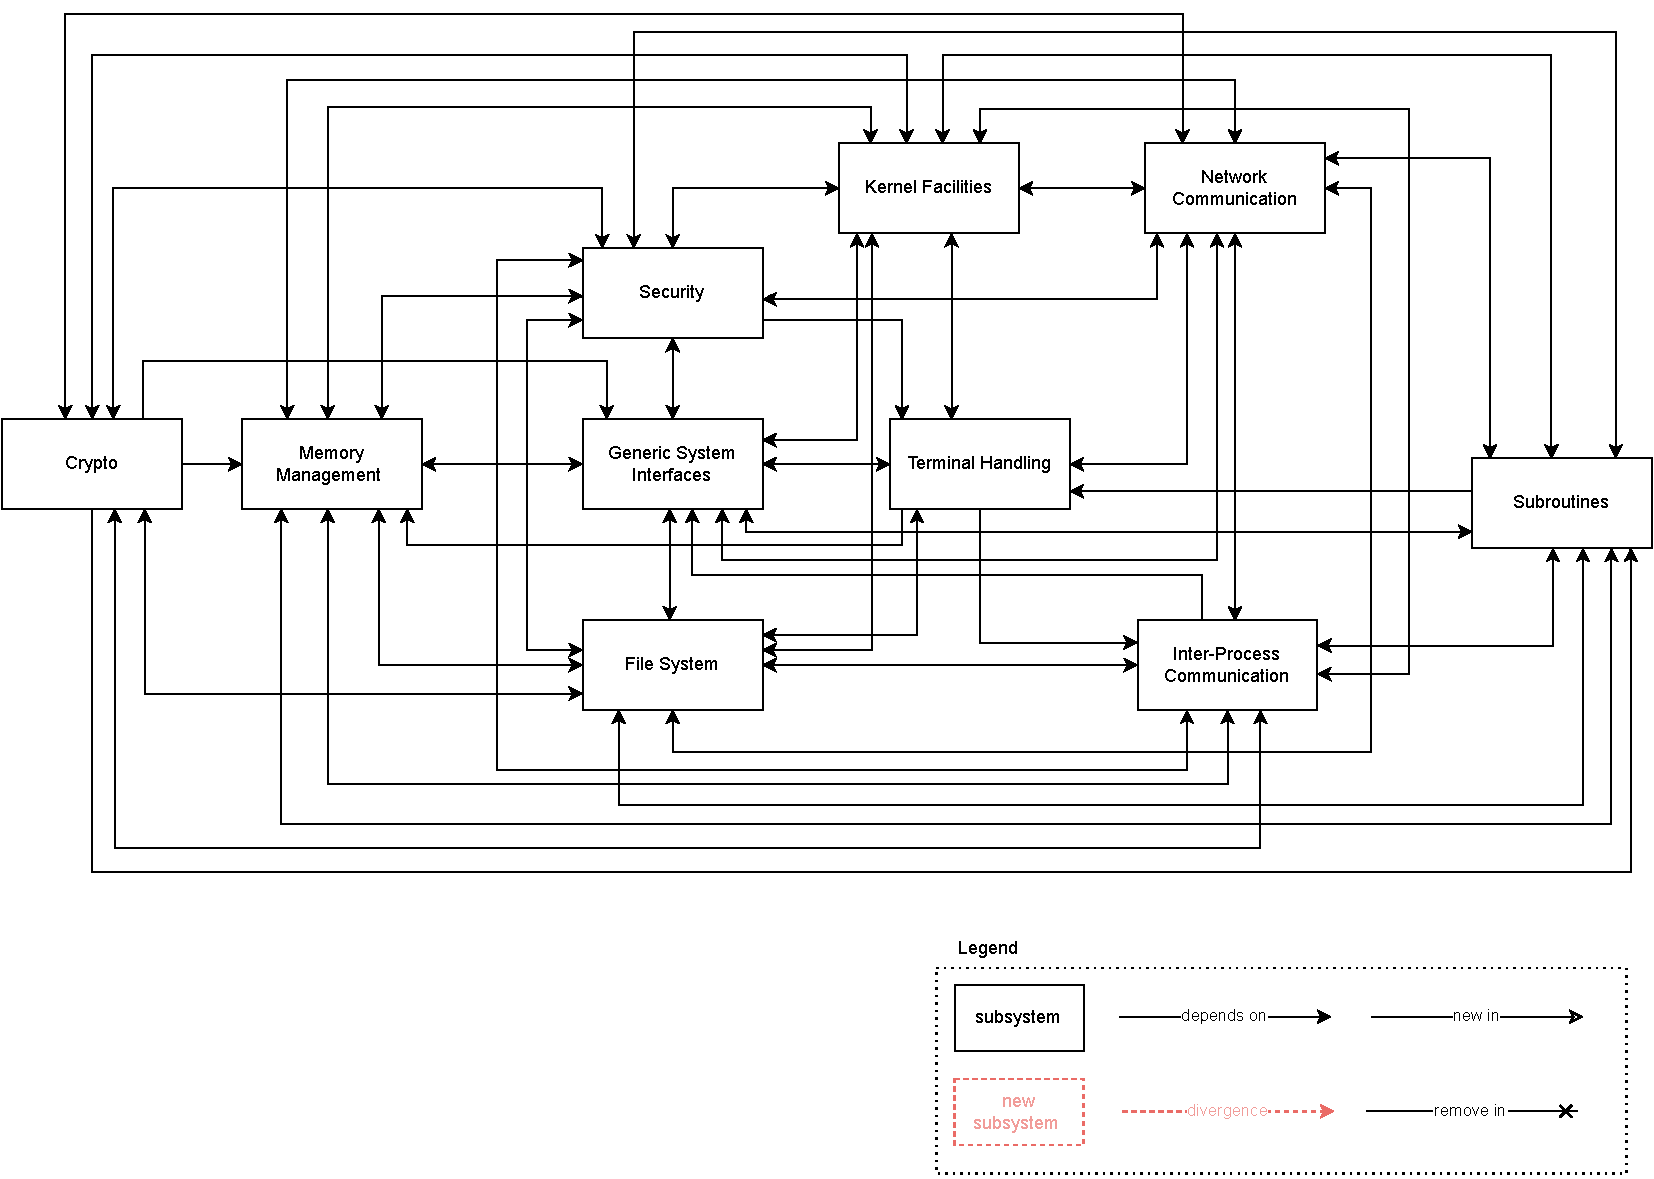
\includegraphics[width = 450pt]{assets/architecture_diagrams/current-concrete-architecture.pdf}
	\caption{Current Concrete Architecture}
\end{figure}

\begin{figure}[!htb]
	\center
	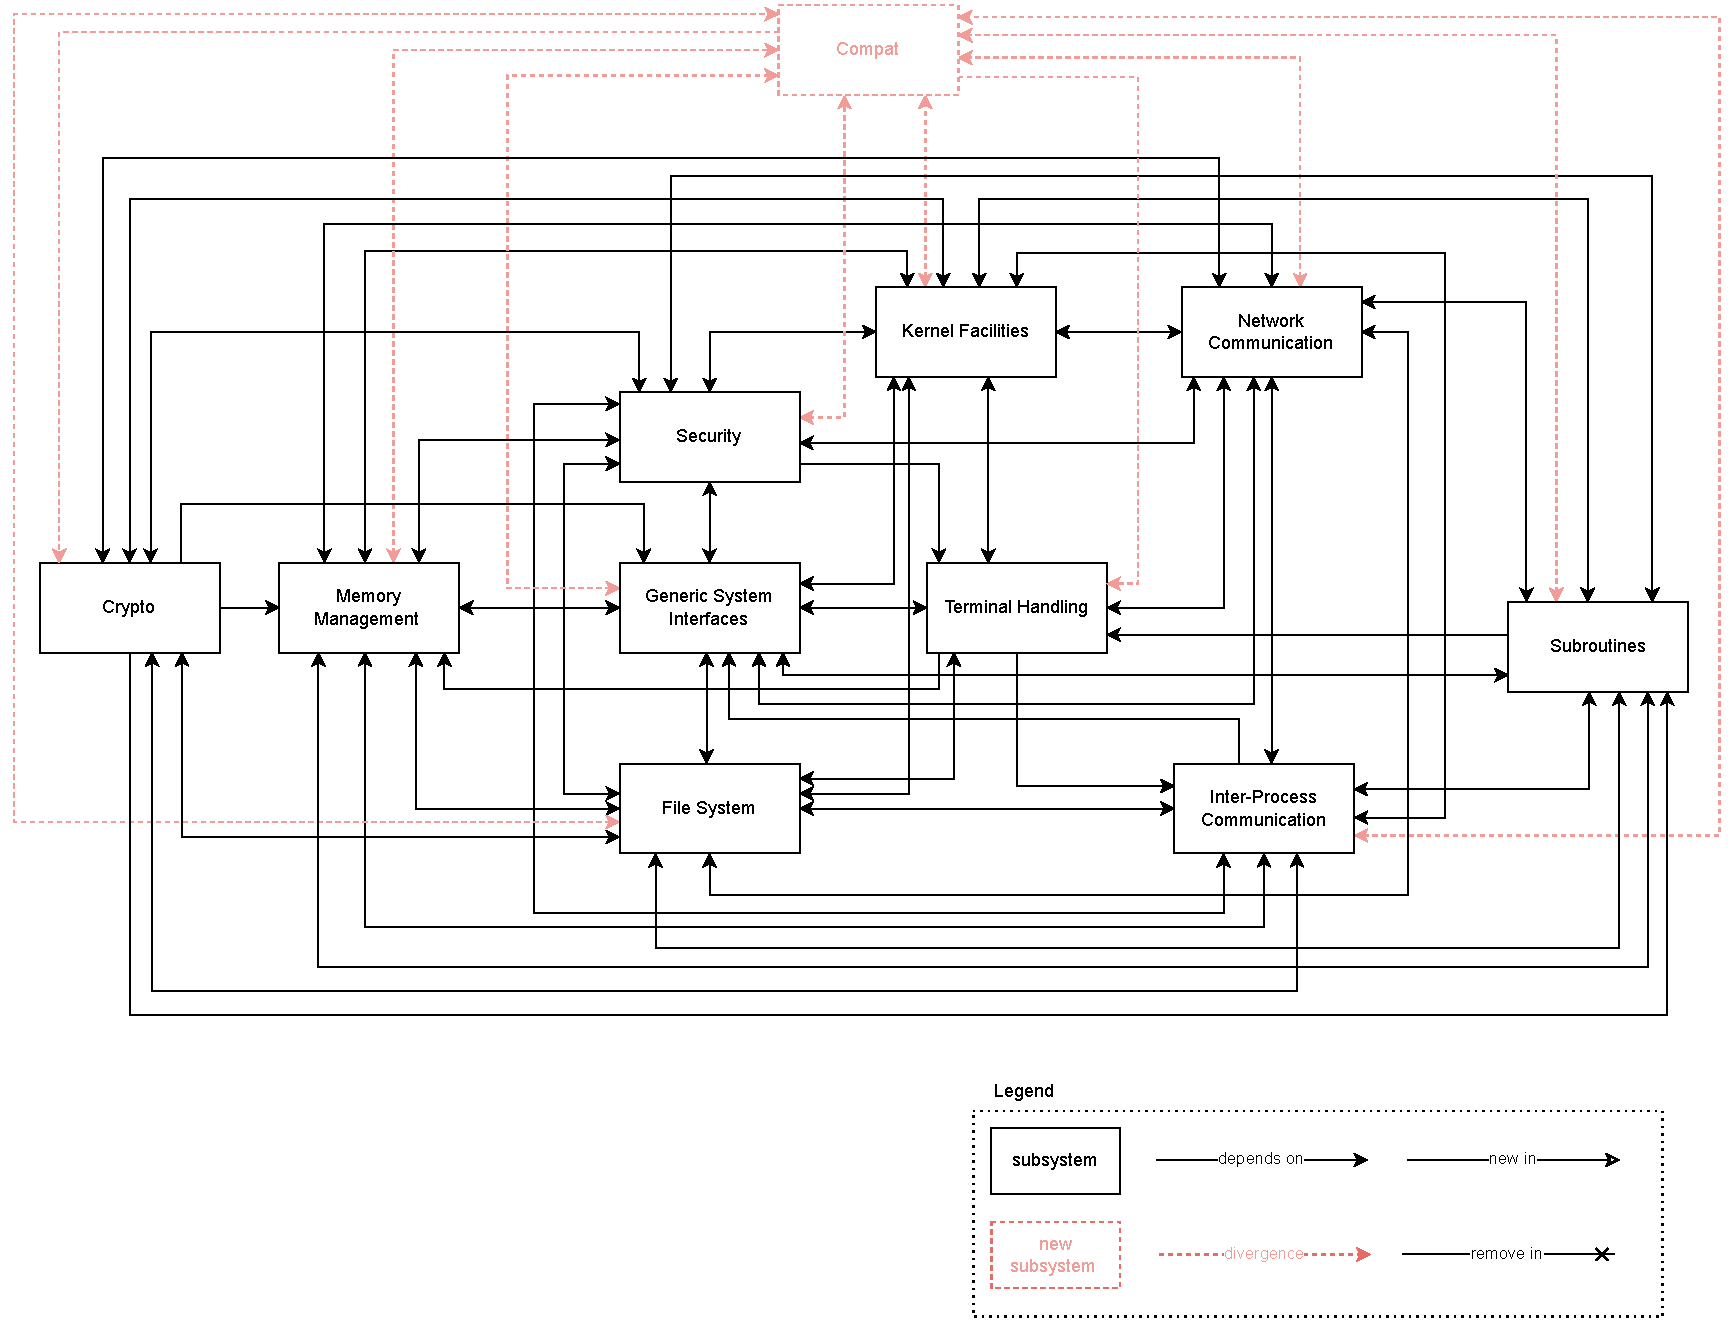
\includegraphics[width = 450pt]{assets/architecture_diagrams/enhanced-concrete-architecture.pdf}
	\caption{Enhanced Concrete Architecture}
\end{figure}

\subsection{Flagged Files}

The proposed enhancement to the Linuxulator subsystem in FreeBSD will significantly impact the system's directory structure. Firstly, the Linuxulator subsystem, which provides a Linux kernel interface for emulation, will be extended to include support for jails. This will introduce a new way for users to leverage FreeBSD's native containerization technology while running Linux applications like Docker.
As a result, the impacted directories include:
\begin{itemize}
	\item \code{sys/compat/linux}
	\item \code{sys/compat/linsysfs}
\end{itemize}

\code{sys/compat/linux} provides binary compatibility files for Linux, while the \code{sys/compat/linsysfs} provides file system emulation for \code{cgroups}. The proposed enhancement will also require changes to specific files, including \code{sys/compat/linux/linux\_fork.c} and its \code{linux\_clone3()} method, to provide support for namespaces by enabling the \code{set\_tid} arg.
Once these changes are made, the Linuxulator subsystem will have improved Linux binary compatibility, thanks to the newly added support for cgroups and namespaces. This will enable FreeBSD to run any Linux binary that requires the use of containerization, making it an attractive platform for developers and businesses alike.

\section{Concurrency}
There are two different versions for how threads are handled in version 1 and 2. In version 1, threads are made distinct from processes. This way, one process can consist of multiple threads at a time. It is also possible to change the cgroups memberships of the threads within the process. However, that ability was removed in version 2, because it caused issues in some cases. For instance, all threads in a process shared a single address space, which caused issues for the memory controller, because it makes no sense to split threads across multiple memory cgroups. That ability was brought back in version 2's thread mode.

In version 2, it has two restrictions imposed on it. One of them is no thread-granularity control, meaning that all threads of a process must belong to the same cgroup. Another restriction is no internal processes, meaning that a cgroup cannot have member processes while controlling child cgroups at the same time. In some cases, it makes sense to have thread-granularity control, such as the CPU controller, so that ability was brought back in the form of thread mode.

Thread mode has several abilities. One is the ability to create threaded subtrees where the threads of a given process are spread across multiple cgroups inside the tree. Another is a new feature called threaded controllers, which can distribute resources across the cgroups in a subtree. Also, the restriction for no internal processes is relaxed. Now, a cgroup can have its own threads and manage child cgroups at the same time.
\clearpage

\section{Use Cases}
\subsection{Docker}
An important use case of our enhancement is the use of an industry standard tool, Docker. Docker does not work without \code{namespace} and \code{cgroup} functionality and our compatibility enhancement would allow these types of applications to run on FreeBSD. Docker and similar containerization engines are widely used in distributed systems within the industry and the diagram below covers the process of emulating \code{namespace} and \code{cgroup} functionality in FreeBSD.
\begin{figure}[!htb]
	\center
	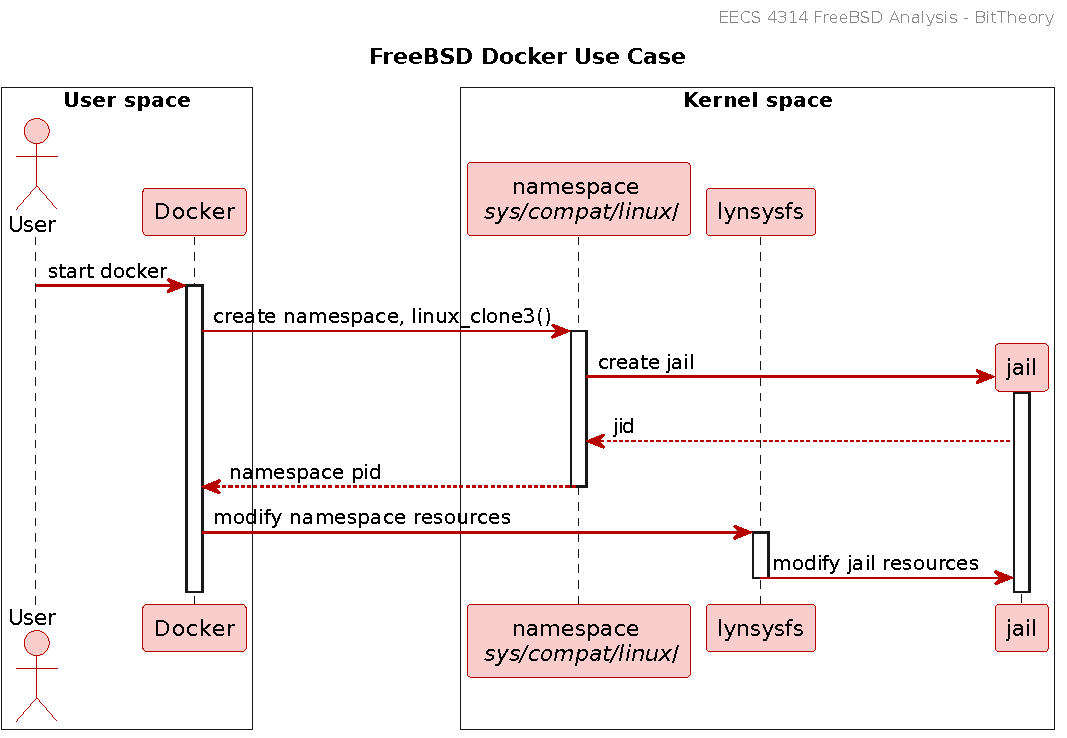
\includegraphics[width = 500pt]{assets/sequence_diagrams/docker.pdf}
	\caption{Docker use case using enhanced state.}
\end{figure}
\clearpage

\section{Risks \& Limitations}
Although the proposed enhancement will lead to improving the overall operating system with better compatibility with Linux, it is still significant to examine how it would potentially affect other factors. For the section, we will observe the risks and limitations from three perspectives: Security, Maintainability, and Performance.

\subsection{Security}
One of the major concerns people would consider when they use containers is leaks of files and resources between the objects. Containers without complete separations would lead to poor efficiency for developments. However, it would not be a concern for this enhancement at this time because this proposed enhancement is based on existing functions and features. For example, to make \texttt{namespace}'s functions work correctly on FreeBSD, we utilize the existed \texttt{clone()} system call, which Linuxulator supports, instead of introducing a completely new idea into the system. Moreover, the mechanism of containers, which will be necessary for the namespace functionality, are from Jails. Jails is a virtual-machine-like containerization tool, completely separating users and processes from the space outside of a Jail \cite{jail}. Therefore, utilizing it as part of the enhancement's functionalities would keep the system secure.

\subsection{Maintainability}
It might be an issue to maintain our proposed enhancement simply because of the relatively small population of contributors who actively support FreeBSD overall. As proof, only several-thousands of developers involve in FreeBSD development \cite{freebsd}. On the other hand, over 10,000 developers contribute in Linux more actively and frequently \cite{linux}. It is possible that the failure of implementation on native Docker development in the past is also due to this factor. Moreover, as there are already existing developed or developing implementations that can support Linux compatibility on FreeBSD, there might not be enough developers interested in or encouraged to maintain this new enhancement in the future. One of the existing implementations is runj, which follows the basics of runc for Linux \cite{runj}.

\subsection{Performance}
This aspect would be challenging to estimate as there is no existing case of internal usage of Jails. As explained earlier in this report, our idea of the enhancement is to create the same functionalities as unsupported Linux features, particularly \texttt{cgroups} and \texttt{namespaces}. Although the enhancement involves modifying the existing functions to add a new parameter feature and introducing fully built container system for isolations, it is still possible that the system will not work as it does by itself.

\section{Conclusion}
In conclusion, the proposed enhancement to extend the linuxulator subsystem in FreeBSD has the potential to significantly improve Linux binary compatibility on FreeBSD. Through a detailed analysis of the benefits, architectural impact, and use cases/sequence diagrams, the proposal demonstrates promising prospects for the FreeBSD operating system and its users.

The enhancement allows for improved compatibility with Linux binaries, particularly for containerization platforms like Docker. This will provide FreeBSD users with access to a wider range of applications and a more seamless deployment and management experience.

The benefits of this enhancement are numerous. As mentioned throughout this report, it would improve compatibility with Linux binaries, enabling FreeBSD to support a wider range of applications and services. This increased compatibility would make FreeBSD more attractive to stakeholders, developers and users who rely on Linux-specific applications, potentially expanding the user base and fostering further development.

In addition, implementing cgroups and namespaces support would not only enhance resource management and process isolation within the operating system (which would consequently optimise performance, allocate resources more efficiently, and ensure better isolation between processes), but would also facilitate its integration with Docker. This would further broaden FreeBSD's appeal and applicability in various use cases, from personal computing to large-scale data centres.

While there are some limitations and risks associated with this enhancement, such as the potential for leaks of files and resources between containers, with proper attention to security and maintainability, these risks can be mitigated. Additionally, the increased interest in the FreeBSD operating system that this enhancement may generate could result in additional contributions to the open-source community and further improvements to the operating system in the future.

In summary, extending the linuxulator subsystem in FreeBSD to provide interfaces for cgroups and namespaces using jails internally offers numerous benefits, including improved Linux binary compatibility, enhanced resource management and process isolation, and better integration with containerization technologies. However, it is essential to acknowledge the limitations and challenges associated with the proposed enhancement that will increase the overall system's complexity. By carefully considering these factors and mitigating the identified challenges, the proposed enhancement has the potential to bring significant value to the FreeBSD operating system and its users.


\section{Lessons Learned}

\textbf{Importance of compatibility between operating systems:}  Enhancements that improve compatibility with other operating systems can significantly expand the range of applications and tools available to users, making an operating system more versatile and attractive. By ensuring compatibility, an operating system can also be used more easily in a variety of environments and integrated more easily with other systems.

\textbf{Different methods of containerization in Linux and FreeBSD:} As we analysed the FreeBSD Operating System to look for potential enhancement proposals, we learned about different methods of containerization technologies in both Linux and FreeBSD. Containerization is a popular technology used for deploying and managing applications. It was learnt that the methods used for containerization differ between Linux and FreeBSD, with jails being the preferred method in FreeBSD. Understanding these differences is important for making informed decisions about how to add support for features such as cgroups and namespaces.

\textbf{Security, maintainability, and performance are potential drawbacks of our proposal:} Enhancements that introduce new functionality or change the architecture of an operating system can also introduce potential risks and challenges by increasing it's overall complexity. It is important to carefully consider the potential drawbacks of any proposed enhancement and develop strategies to mitigate risks related to security, maintainability, and performance.

\textbf{Architectural analysis is crucial the implementation of such enhancement feature:} Enhancements that involve changes to an operating system's architecture require careful analysis to ensure that they are technically feasible, maintainable, and efficient. By performing a thorough analysis of the architecture and potential impacts of a proposed enhancement, stakeholders can make informed decisions about the potential implementation of features that could potentially add value to the overall system.

\textbf{Collaboration with stakeholders is crucial for successful enhancements:} Enhancements that involve significant changes to an operating system require collaboration with a range of stakeholders, including developers, users, and companies that may be impacted by the changes, such as Docker in this case. By engaging with stakeholders and soliciting feedback throughout the development process, it is possible to build enhancements that meet the needs of a wide range of users and maximise the benefits of the enhancement for all stakeholders involved.
\clearpage

\section{Data Dictionary}
\begin{itemize}
	\item {Linuxulator (Linux Emulation): A technique to Linux binaries on FreeBSD without any modifications \cite{linuxulator}}
	\item {cgroups: One of the features in Linux, which sets aside resources within namespaces for other usages}
	\item {namespaces: One of the features in Linux, which creates several numbers of completely separated spaces within the operating system}
	\item {Docker: A technique based on both hypervisor-based and containerized virtualizations}
	\item {runj: A Docker-like tool which supports Jails based on the OCI runtime specifications}
	\item {runc: A Linux tool which manages container systems based on the OCI specifications}
	\item {Jails: A FreeBSD tool which follows the functionalities of the containerized virtualization}
\end{itemize}

\section{Naming Conventions}
\begin{itemize}
	\item {cgroup: Control group}
	\item {OCI: Open Container Initiative}
\end{itemize}
\clearpage

\begin{thebibliography}{00}
	\bibitem{cgroups} Cgroups(7) - Linux Manual Page, \href{https://man7.org/linux/man-pages/man7/cgroups.7.html}{https://man7.org/linux/man-pages/man7/cgroups.7.html}.
	\bibitem{linuxbinarycompat} “Chapter 11. Linux Binary Compatibility.” FreeBSD Documentation Portal, \href{https://docs.freebsd.org/en/books/handbook/linuxemu/}{https://docs.freebsd.org/en/books/handbook/linuxemu/}.
	\bibitem{clone} Clone(2) - Linux Manual Page, \href{https://man7.org/linux/man-pages/man2/clone.2.html}{https://man7.org/linux/man-pages/man2/clone.2.html}.
	\bibitem{jail} Delgado, Sergio  Carlavilla. “Chapter 16. Jails.” FreeBSD Documentation Portal, 4 Mar. 2023, \href{https://docs.freebsd.org/en/books/handbook/jails/}{https://docs.freebsd.org/en/books/handbook/jails/}.
	\bibitem{freebsd} Freebsd. “FreeBSD/FreeBSD-Src$\,\colon\,$ The Freebsd Src Tree.” GitHub, 1993, \href{https://github.com/freebsd/freebsd-src}{https://github.com/freebsd/freebsd-src}.
	\bibitem{linsysfs} “FreeBSD Manual Pages.” Linsysfs, \href{https://man.freebsd.org/cgi/man.cgi?linsysfs}{https://man.freebsd.org/cgi/man.cgi?linsysfs}.
	\bibitem{runj} Karp, Samuel. “Samuelkarp/Runj$\,\colon\,$ Runj.” GitHub, 2020, \href{https://github.com/samuelkarp/runj}{https://github.com/samuelkarp/runj}.
	\bibitem{linuxulator} “Linuxulator.” Edited by Graham Perrin, Linuxulator - FreeBSD Wiki, 29 Jan. 2023, \href{https://wiki.freebsd.org/Linuxulator}{https://wiki.freebsd.org/Linuxulator}.
	\bibitem{linux} Torvalds, Linus. “Torvalds/Linux$\,\colon\,$ Linux Kernel Source Tree.” GitHub, 2002, \href{https://github.com/torvalds/linux}{https://github.com/torvalds/linux}.



\end{thebibliography}
\end{document}
